\documentclass[preview]{standalone}
\usepackage[right=-16in]{geometry}
\usepackage{tikz}
% \usepackage{xcolor}
\usetikzlibrary{arrows,automata,calc,decorations.pathreplacing}
% \usepackage[latin1]{inputenc}

% Show PSK rules
\newif\ifpsk
\pskfalse

% Show session resumption
\newif\ifdrawres
% \drawrestrue
\drawresfalse

% Show post-handshake rules
\newif\ifposths
%\posthstrue
\posthsfalse

% Show 0-RTT rules
\newif\ifzerortt
% \zerortttrue
\zerorttfalse

% Show application data
\newif\ifrecord
\recordtrue

\begin{document}
\begin{figure}
% \begin{center}
  
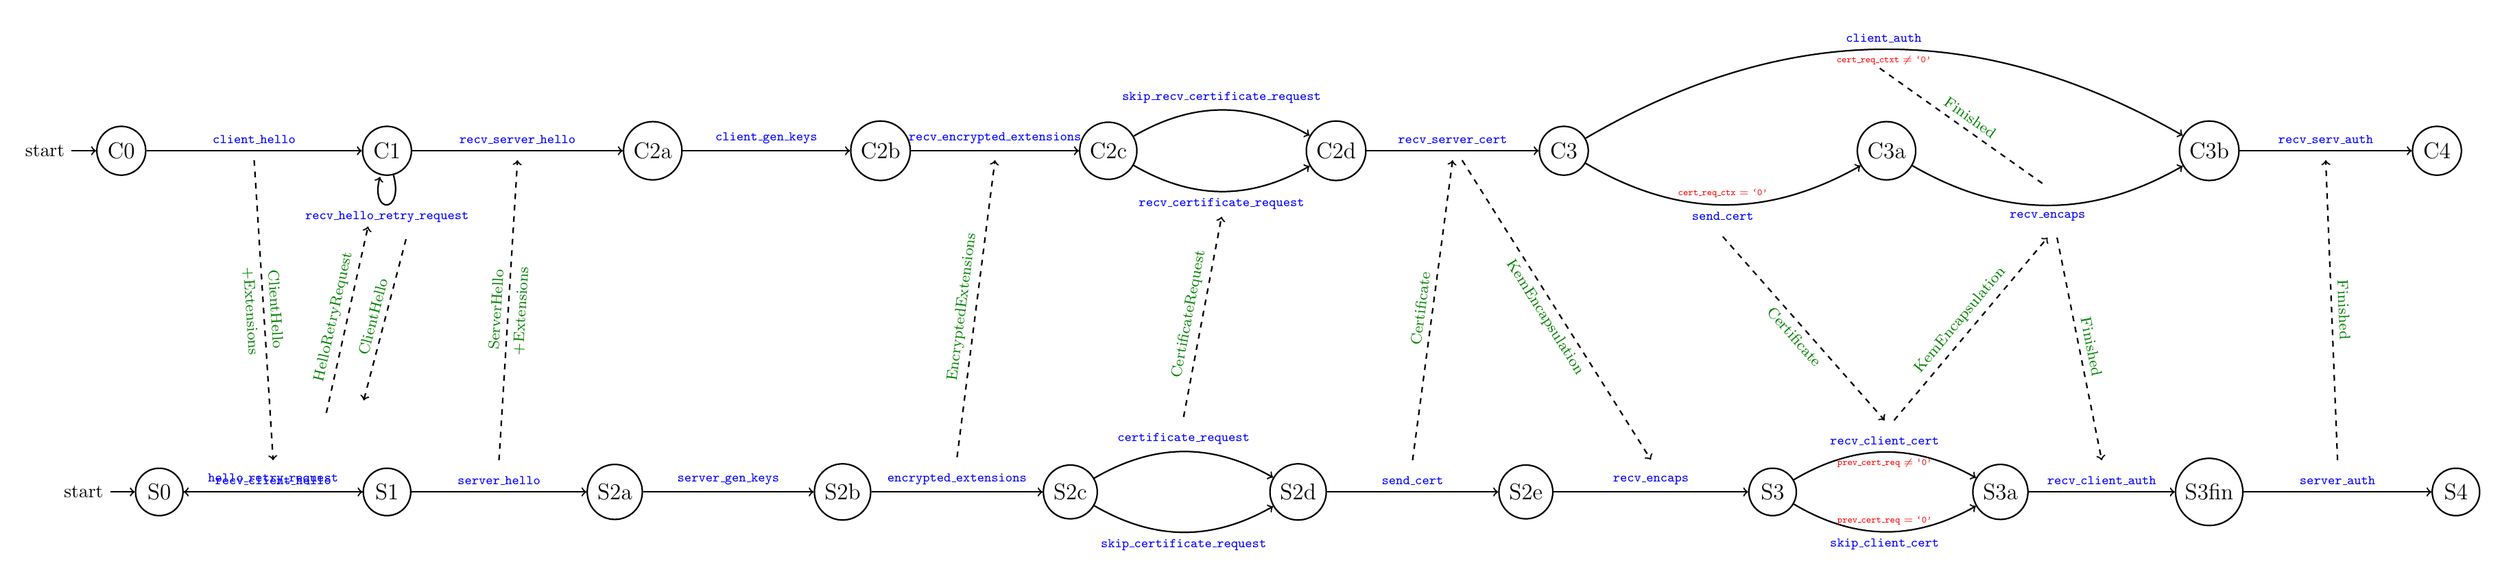
\begin{tikzpicture}[->, node distance=120, thick]
  \tikzstyle{every state}=[font=\large]
  \tikzstyle{rule} = [color=blue, font=\ttfamily\scriptsize]
  \tikzstyle{precon} = [color=red, font=\ttfamily\tiny, text width=75, align=center]
  \tikzstyle{msg} = [color=green!50!black, font=\footnotesize, text width=80, align=center]
  \tikzstyle{msg edge} = [dashed] 

  % Client states
  \node[initial,state] (C0) {C0};
  \node[state] (C1) [right of=C0, xshift=20] {C1};
  \node[state] (C2a) [right of=C1, xshift=20] {C2a};
  \node[state] (C2b) [right of=C2a] {C2b};
  \node[state] (C2c) [right of=C2b] {C2c};
  \node[state] (C2d) [right of=C2c] {C2d};
  \node[state] (C3) [right of=C2d] {C3};
  \node[state] (C3a) [right of=C3, node distance=170] {C3a};
  \node[state] (C3b) [right of=C3a, node distance=170] {C3b};
  \node[state] (C4) [right of=C3b] {C4};

  % Server states
  \node[initial,state] (S0) [below of=C0, node distance=180, xshift=20] {S0};
  \node[state] (S1) [right of=S0] {S1};
  \node[state] (S2a) [right of=S1] {S2a};
  \node[state] (S2b) [right of=S2a] {S2b};
  \node[state] (S2c) [right of=S2b] {S2c};
  \node[state] (S2d) [right of=S2c] {S2d};
  \node[state] (S2e) [right of=S2d] {S2e};
  \node[state] (S3) [right of=S2e, xshift=10] {S3};
  \node[state] (S3a) [right of=S3] {S3a};
  \node[state] (S3fin) [right of=S3a, xshift=-10] {S3fin};
  \node[state] (S4) [right of=S3fin, xshift=10] {S4};

  \ifpsk
    % Initial PSK states
    \node (CPSK) [above of=C0, font=\small, node distance=50] {ClientPSK};
    \node (SPSK) [below of=S0, font=\small, node distance=50] {ServerPSK};
  \fi

  \ifposths
    % States for post-hs authentication
    \node[state] (S4_req) [right of=S4, xshift=-40] {S4};
    \node[state] (C4_req) [right of=C4, xshift=-20] {C4};
    \node[state] (C4_cert)[right of=C4_req] {C4};
    \node[state] (S4_cert)[right of=S4_req] {S4};
    \node[state] (C4_end) [right of=C4_cert] {C4};
    \node[state] (S4_end) [right of=S4_cert] {S4};

    % States for KeyUpdate
    \node[state] (S4_up_req) [right of=S4_end, xshift=-30] {S4};
    \node[state] (C4_up_recv) [right of=C4_end, xshift=30] {C4};
    \node[state] (C4_up_fin) [right of=C4_up_recv] {C4};
    \node[state] (S4_up_fin) [right of=S4_up_req] {S4};
    \node[state] (S4_up_end) [right of=S4_up_fin] {S4};
  \fi

    % Client basic rules
    \path 
      \ifpsk
        (C0) edge [bend right] node [below, rule] (ch) {client\_hello} (C1)
        (C1) edge [bend right] node [below, rule] (rsh) {recv\_server\_hello} (C2a)
        (C2d) edge [bend right] node [below, rule] (rsa) {recv\_server\_cert} (C3)
      \else
        (C0) edge [] node [above, rule] (ch) {client\_hello} (C1)
        (C1) edge [] node [above, rule] (rsh) {recv\_server\_hello} (C2a)
        (C2d) edge [] node [above, rule] (rsc) {recv\_server\_cert} (C3)
      \fi
      \ifzerortt
        (C1) edge [loop below] node [below, rule] (zra) {zero\_rtt\_auth} (C1)
      \else
        (C1) edge [loop below] node [below, rule] (rhrr) {recv\_hello\_retry\_request} (C1)
      \fi
        (C2a) edge [] node [above, rule] {client\_gen\_keys} (C2b)
        (C2b) edge [] node [above, rule] (ree) {recv\_encrypted\_extensions} (C2c)
        (C2c) edge [bend right] node [below, rule] (rcr) {recv\_certificate\_request} (C2d)
        (C2c) edge [bend left] node [above, rule] {skip\_recv\_certificate\_request} (C2d)
        (C3) edge [bend left] node [above, rule] (ca1) {client\_auth} node [below, precon] {cert\_req\_ctxt $\neq$ `0'} (C3b)
        (C3) edge [bend right] node [below, rule] (cacrt) {send\_cert} node [above, precon] {cert\_req\_ctx $=$ `0'} (C3a)
        (C3a) edge [bend right] node [below, rule] (cact) {recv\_encaps} (C3b)
        (C3b) edge [] node [above, rule] (rsa) {recv\_serv\_auth} (C4)
        ;

    % Server basic rules
    \path 
      \ifpsk
        (S0) edge [bend left] node [above, rule] (rch) {recv\_client\_hello} (S1)
        (S1) edge [bend left] node [above, rule] (sh) {server\_hello} (S2a)
        (S2d) edge [bend left] node [above, rule] (sa) {server\_auth} (S3)
      \else
        (S0) edge [] node [above, rule] (rch) {recv\_client\_hello} (S1)
        (S1) edge [] node [above, rule] (sh) {server\_hello} (S2a)
        (S3fin) edge [] node [above, rule] (sa) {server\_auth} (S4)
      \fi
      \ifzerortt
        (S1) edge [loop above] node [above, rule] (rzra) {recv\_zero\_rtt\_auth} (S1)
      \else
        (S1) edge [] node [above, rule] (hrr) {hello\_retry\_request} (S0)
      \fi
        (S2a) edge [] node [above, rule] {server\_gen\_keys} (S2b)
        (S2b) edge [] node [above, rule] (ee) {encrypted\_extensions} (S2c)
        (S2c) edge [bend left] node [above, rule] (cr) {certificate\_request} (S2d)
        (S2c) edge [bend right] node [below, rule] {skip\_certificate\_request} (S2d)
        (S2d) edge [] node [above, rule] (scrt) {send\_cert} (S2e)
        (S2e) edge [] node [above, rule] (rct) {recv\_encaps} (S3)
        (S3) edge [bend right] node [below, rule] {skip\_client\_cert} node [above, precon] {prev\_cert\_req $=$ `0'} (S3a)
        (S3) edge [bend left] node [above, rule] (rccrt) {recv\_client\_cert} node [below, precon] {prev\_cert\_req $\neq$ `0'} (S3a)
        (S3a) edge [] node [above, rule] (rca) {recv\_client\_auth} (S3fin)
        ;

    % Messages sent
    \path
        % ClientHello
        ([yshift=-5]ch.south) edge [msg edge] node [sloped, above, msg] {ClientHello}
                                              node [sloped, below, msg] {+Extensions} ([yshift=5]rch.north)

      \ifzerortt
        % ClientAuth
        ([yshift=-5]zra.250) edge [msg edge] node [sloped, above, msg] {Finished} ([yshift=5]rzra.80)
      \else
        % HelloRetryRequest
        ([yshift=35, xshift=-10]hrr.0) edge [msg edge] node [sloped, above, msg] {HelloRetryRequest} ([yshift=-5, xshift=-10]rhrr)
        ([yshift=-5, xshift=10]rhrr.south) edge [msg edge] node [sloped, above, msg] {ClientHello} ([yshift=35, xshift=10]hrr.10)
      \fi
        % ServerHello
        ([yshift=5]sh.north) edge [msg edge] node [sloped, above, msg] {ServerHello}
                                             node [sloped, below, msg] {+Extensions} ([yshift=-5]rsh.south)
        % EncryptedExtensions
        ([yshift=5]ee.north) edge [msg edge] node [sloped, above, msg] {EncryptedExtensions} ([yshift=-5]ree.south)
        % CertificateRequest
        ([yshift=5]cr.north) edge [msg edge] node [sloped, above, msg] {CertificateRequest} (rcr.south)
        % ServerAuth
        ([yshift=5]scrt.north) edge [msg edge] node [sloped, above, msg] {Certificate} ([yshift=-5]rsc.south)
        ([yshift=-5,xshift=5]rsc.south) edge [msg edge] node [sloped, below, msg] {KemEncapsulation} ([yshift=5]rct.north)
        ([yshift=5]sa.north) edge [msg edge] node [sloped, above, msg] {Finished} ([yshift=-5]rsa.south)
        % ClientAuth
        ([yshift=-5]cacrt.south) edge [msg edge] node [sloped, below, msg] {Certificate} ([yshift=5]rccrt.north)
        ([yshift=5,xshift=5]rccrt.north) edge [msg edge] node [sloped, above, msg] {KemEncapsulation} ([yshift=-5]cact.south)
        ([yshift=-5,xshift=5]cact.south) edge [msg edge] node [sloped, above, msg] {Finished} ([yshift=5]rca.north)
        ([yshift=-10]ca1.250) edge [-, msg edge] node [sloped, above, msg] {Finished} ([yshift=10]cact.95)
        %([yshift=-10]rca.300) edge [->, msg edge] ([yshift=10]rca.45)
        ;

    \ifpsk
    % PSK Rules/messages
    \path 
        % Client/ServerPSK to initial state
        (CPSK) edge [bend right] (C0)
        (SPSK) edge [bend left] (S0)
        % NewSessionTicket
        (C4) edge [loop below] node [anchor=150, rule] (rnst) {recv\_new\_session\_ticket} (C4)
        (S4) edge [loop above] node [above, rule] (nst) {new\_session\_ticket} (S4)
        ([yshift=5]nst.150) edge [msg edge] node [sloped, above, msg] {NewSessionTicket} ([yshift=-5]rnst.290)
        % ClientHelloPSK
        (C0) edge [bend left] node [above, rule] (ch_psk) {client\_hello\_psk} (C1)
        (S0) edge [bend right] node [below, rule] (rch_psk) {recv\_client\_hello\_psk} (S1)
        ([yshift=-5]ch_psk.230) edge [-, msg edge] ([yshift=5]ch.110)
        ([yshift=-5]rch.300) edge [->, msg edge] ([yshift=5]rch_psk.45)
        % ServerHelloPSK
        (S1) edge [] node [above, rule, yshift=-3] (sh_psk) {server\_hello\_psk} (S2a)
        (S1) edge [bend right] node [below, rule] (sh_psk_dhe) {server\_hello\_psk\_dhe}
                               node [above, precon] {ke\_mode = \mbox{$\langle$ `psk\_dhe\_ke', `psk\_ke' $\rangle$}} (S2a)
        (C1) edge [] node [above, rule, yshift=-3] (rsh_psk) {recv\_server\_hello\_psk} (C2a)
        (C1) edge [bend left] node [above, rule] (rsh_psk_dhe) {recv\_server\_hello\_psk\_dhe}
                              node [below, precon] {ke\_mode = \mbox{$\langle$ `psk\_dhe\_ke', `psk\_ke' $\rangle$}} (C2a)
        ([yshift=5]sh_psk_dhe.120) edge [-, msg edge] ([yshift=-5]sh_psk.245)
        ([yshift=0]sh_psk.100) edge [-, msg edge] ([yshift=-3]sh.265)
        ([yshift=5]rsh.80) edge [->, msg edge] ([yshift=0]rsh_psk.290)
        ([yshift=0]rsh_psk.65) edge [->, msg edge] ([yshift=-3]rsh_psk_dhe.300)
        % ServerAuthPSK
        (C2d) edge [bend left] node [above, rule] (rsa_psk) {recv\_server\_auth\_psk}
                                node [below, precon] {auth\_mode = `psk\_auth'} (C3)
        (C2d) edge [bend right, opacity=0] node [above, precon, opacity=100] { auth\_mode $\in$ \{`psk\_sign\_auth', `0'\}} (C3)
        (S2d) edge [bend right] node [below, rule] (sa_psk) {server\_auth\_psk}
                                node [above, precon] {auth\_mode = `psk\_auth'} (S3)
        (S2d) edge [bend left, opacity=0] node [below, precon, opacity=100] { auth\_mode $\in$ \{`psk\_sign\_auth', `0'\}} (S3)
        ([yshift=5]sa.north) edge [msg edge] node [sloped, below, msg] {Finished} ([yshift=-5]rsa.south)
        ([yshift=5]sa.north) edge [msg edge] node [sloped, below, msg] {Finished} ([yshift=-5]rsa.south)
        ([yshift=10]sa_psk.130) edge [-, msg edge] ([yshift=-15]sa.245)
        ([yshift=15]rsa.70) edge [->, msg edge] ([yshift=-10]rsa_psk.300)

      \ifdrawres
        % Edge connecting new session ticket to initial PSK
        (rnst.east) edge [dotted, out=45, in=45, looseness=0.5] (CPSK)
        (nst.east) edge [dotted, out=315, in=300, looseness=0.5] (SPSK)
      \fi
        ;
    \fi


    \ifzerortt
      \node (CZRS) [above of=C1, xshift=20, node distance=50, text width=70, align=center] {ZeroRTTStream \mbox{\scriptsize(after \texttt{zero\_rtt\_auth})}};
      \node (SZRS) [below of=S1, xshift=20, node distance=50, text width=70, align=center] {ZeroRTTStream \mbox{\scriptsize(after \texttt{recv\_zero\_rtt\_auth})}};
      \path 
          (C1) edge [bend left] (CZRS)
          (S1) edge [bend right] (SZRS);
    \fi

    \ifposths
      \path
          % Continue state
          (C4) edge [dotted] (C4_req)
          (S4) edge [dotted] (S4_req)
          (C4_req) edge [loop above, dotted] (C4_req)
          (C4_cert) edge [loop above, dotted] (C4_cert)
          (C4_end) edge [loop above, dotted] (C4_end)
          (S4_req) edge [loop below, dotted] (S4_req)
          (S4_cert) edge [loop below, dotted] (S4_cert)
          (S4_end) edge [loop below, dotted] (S4_end)
          (C4_end) edge [dotted] (C4_up_recv)
          (S4_end) edge [dotted] (S4_up_req)
          (C4_up_recv) edge [loop above, dotted] (C4_up_recv)
          % (C4_up_fin) edge [loop above, dotted] (C4_up_fin)
          (S4_up_req) edge [loop below, dotted] (S4_up_req)
          (S4_up_fin) edge [loop below, dotted] (S4_up_recv)
          % (S4_up_end) edge [loop below, dotted] (S4_up_end)
          (S4_up_end) edge [dotted] ([xshift=60]S4_up_end)
          (C4_up_fin) edge [dotted] ([xshift=60]C4_up_fin)

          % Request post-hs authentication
          (S4_req) edge [] node [above, rule] (crp) {certificate\_request\_post} (S4_cert)
          (C4_req) edge [] node [above, rule] (rcrp) {recv\_certificate\_request\_post } (C4_cert)
          ([yshift=5]crp.135) edge [msg edge] node [sloped, above, msg] {CertificateRequest} ([yshift=-5]rcrp.330)

          % Send auth
          (C4_cert) edge [] node [above, rule] (cap) {client\_auth\_post} (C4_end)
          (S4_cert) edge [] node [above, rule] (rcap) {recv\_client\_auth\_post} (S4_end)
          ([yshift=-5]cap.200) edge [msg edge] node [sloped, above, msg] {Certificate \mbox{CertificateVerify} Finished} ([yshift=5]rcap.45)

          % Request key update
          (S4_up_req) edge [] node [above, rule] (urs) {update\_req\_server} (S4_up_fin)
          (C4_up_recv) edge [] node [above, rule] (urc) {update\_recv\_client} (C4_up_fin)
          ([yshift=5]urs.135) edge [msg edge] node [sloped, above, msg] {KeyUpdate} ([yshift=-5]urc.200)

          % Recieve and send key update
          (S4_up_fin) edge [] node [above, rule] (ufs) {update\_fin\_server} (S4_up_end)
          ([yshift=-5]urc.330) edge [msg edge] node [sloped, above, msg] {KeyUpdate} ([yshift=5]ufs.45)

          ;
    \fi

    \ifrecord
      % Display where TLS stream is created for application data.
      \ifpsk
        \node (SSendTLS) [below of=sa_psk, xshift=20, node distance=50] {SendStream};
        \node (CRecvTLS) [above of=rsa_psk, xshift=20, node distance=50] {RecvStream};
        \node (SRecvTLS) [below of=rca, xshift=20, node distance=50] {RecvStream};
        \node (CSendTLS) [above of=cac, xshift=20, node distance=50] {SendStream};
        \path 
          (rsa_psk) edge [bend left] (CRecvTLS)
          (sa_psk) edge [bend right] (SSendTLS)
          (cac) edge [bend left] (CSendTLS)
          (rca) edge [bend right] (SRecvTLS);
      \else
        \node (SSendTLS) [below of=sa, xshift=20, node distance=50] {SendStream};
        \node (CRecvTLS) [above of=rsa, xshift=20, node distance=50] {RecvStream};
        \node (SRecvTLS) [below of=rca, xshift=20, node distance=50] {RecvStream};
        \node (CSendTLS) [above of=ca1, xshift=20, node distance=50] {SendStream};
        \path 
          (rsa) edge [bend left] (CRecvTLS)
          (sa) edge [bend right] (SSendTLS)
          (ca1) edge [bend left] (CSendTLS)
          (cact.750) edge [bend right] (CSendTLS)
          (rca) edge [bend right] (SRecvTLS);
      \fi

      \ifposths
        \node (CTLS1) [above of=urc, xshift=20, node distance=50] {RecvStream, SendStream};
        \node (STLS1) [below of=urs, xshift=20, node distance=50] {SendStream};
        \node (STLS2) [below of=ufs, xshift=20, node distance=50] {RecvStream};
        \path 
            (urc) edge [bend left] (CTLS1)
            (urs) edge [bend right] (STLS1)
            (ufs) edge [bend right] (STLS2);
      \fi
    \fi

\end{tikzpicture} \\

% \end{center}
% \ifpsk
% \caption{
\hspace{0.5cm}
\fbox{
\begin{minipage}{10cm}
Possible options are:
\begin{itemize}
  \item PSK rules: \ifpsk \textbf{Active} \else \emph{Hidden} \fi
  \item Resumption edge: \ifdrawres \textbf{Active} \else \emph{Hidden} \fi
  \item Record layer: \ifrecord \textbf{Active} \else \emph{Hidden} \fi
  \item 0-RTT rules: \ifzerortt \textbf{Active} \else \emph{Hidden} \fi
  \item Post-handshake rules: \ifposths \textbf{Active} \else \emph{Hidden} \fi
\end{itemize}
\end{minipage} 
}
\hspace{5cm}
\begin{minipage}{20cm}
\textbf{\large State machine for client and server rules.}
\begin{description}
  \item[Nodes] correspond to the client/server state (given by State\_N in the model).
  \item[Edges] represent rules causing transitions between states - written in blue text. 
  \item[Red text] indicates preconditions which must be met for adjacent rule to apply.
  \item[Dashed lines] with green text are for messages sent due to the rule.
  \item[] Where two parallel lines can both send a message, this is indicated by a dashed line connecting the two.
\end{description}
\ifzerortt
Info: HelloRetryRequest rules have been hidden for clarity.
\fi
\end{minipage} 

\end{figure}

\end{document}
